%%This is a very basic article template.
%%There is just one section and two subsections.
\documentclass{article}
\usepackage{graphics}
\usepackage{graphicx}
\usepackage{url}
\usepackage[utf8]{inputenc}
\usepackage[spanish]{babel}
\usepackage{myCoverPage}
\usepackage{fancyhdr}
\usepackage{color}
\usepackage{colortbl}
\usepackage{colourlist}


\usepackage{tocloft}

%If invoked with [final] then fixes and notes will be not shown
\usepackage[final,inline]{fixme}
\usepackage{hyperref}

% configuración del paquete hyperref
\hypersetup{    pdfauthor = {/Elena Mor'on Muela},
		pdftitle = {},
		colorlinks={true},
		pdfstartview={FitV},
		linkcolor={blue4},
		citecolor={blue4},
		urlcolor={blue4}
}




\usepackage[a4paper]{geometry}
\oddsidemargin -0.04cm   % read Lamport p.163
\evensidemargin -0.04cm  % same as oddsidemargin but for left-hand pages

\renewcommand{\CoverPageHeader}{%
    \parbox{\linewidth}{%
        \tiny
   
    }%
}

% Control de lneas viudas y huérfanas
\clubpenalty=100000
\widowpenalty=10000
\displaywidowpenalty=1000
\looseness=1

%-----------------------------------------------------------------------------%
%
% Formato de las cabeceras
%
\pagestyle{fancyplain}

\lhead[
        \fancyplain{}
	    {\textrm{\textbf{\thepage}\hspace{4mm}\small\leftmark}}]
        {\fancyplain{}
        {\textrm{\footnotesize\textcopyright\ GSO}}}
\rhead[
        \fancyplain{}
        {\textrm{\footnotesize\textcopyright\ GSO}}]
        {\fancyplain{}
        {\textrm{\small\rightmark\hspace{4mm}\normalsize\textbf{\thepage}}}}
\cfoot[]{} % En el pie de página no ponemos nada
\renewcommand{\headrulewidth}{0.1mm}

\graphicspath{\resources}
%¿No debería ser Anteproyecto de Trabajo de Fin de Carrera?
\renewcommand{\CPTitle}{\LARGE Anteproyecto de Fin de Grado.\\\huge\sc Aplicación informática para auditorias de Prevención y Blanqueo de Capitales y Financiación del Terrorismo}
\renewcommand{\CPAuthor}{Autor: \ Elena Morón Muela\\Tutor: \'Oscar Garc\'ia
Población}
\renewcommand{\CPDireccion}{Universidad de Alcalá\\Escuela
Politécnica Superior\\Departamento de Automática\\}
%\newcommand{\tituloTFC}{Sistema integrado de información geográfica para la gestión de expropiaciones}
%¿para que sirve la siguiente línea?
%sale un source undefined debajo del email.
\newcommand{\ssh}{\texttt{ssh}}


\begin{document}
\title{Propuesta de Proyecto fin de Carrera}
\pagenumbering{arabic}
\setcounter{page}{2}
\cleardoublepage

\setcounter{tocdepth}{2}
\tableofcontents
\listoffixmes


\section{Introducción}
Este documento presenta el anteproyecto titulado Aplicación informática para auditorias de prevención de blanqueo de capitales y financión del terrorismo. En él se propone el desarrollo de una aplicación informática que ayuda a las labores generales de una empresa de auditorias en la detección de blanqueo de capitales y financión del terrorismo.

La presente Ley de prevención del blanqueo de capitales y financiación del terrorismo tiene por objeto la protección de la integridad del sistema financiero y de otros sectores de actividad económica mediante el establecimiento de obligaciones.

Comenzaremos pot establecer una serie de objetivos, la descripción de trabajo a realizar, organizado en un diagrama de Gantt que muestra el plan de trabajo a seguir, además del plan de trabajo se hablará de metodología que se usará para el desarrollo del proyecto.
Por último una bibliografía para indicar que fuentes han sido utilizadas.  


 


\section{Objetivos y campo de aplicación.}
Los objetivos han movido el desarrollo de este proyecto, se dividen en dos bloques desde el punto de vista de la aplicación. El acceso a la aplicación, permitiendo un acceso multiplataforma a los servicios desde móviles y desktop. El almacenamiento y procesado de la información. 
Para alcanzar estos objetivos será necesario comprender y aplicar adecuadamente varias tecnologías que se describen acontinuación.



\section{Descripción del trabajo}
El trabajo consiste en tres entregables: una memoria explicativa, aplicación javascript basada en angular y una aplicación python basada en django.

Se dispone de dos grandes bloques conocidos como backend y frontend,en la siguiente imagen se muestran con las tecnologias que intervienen en casa uno de ellos.

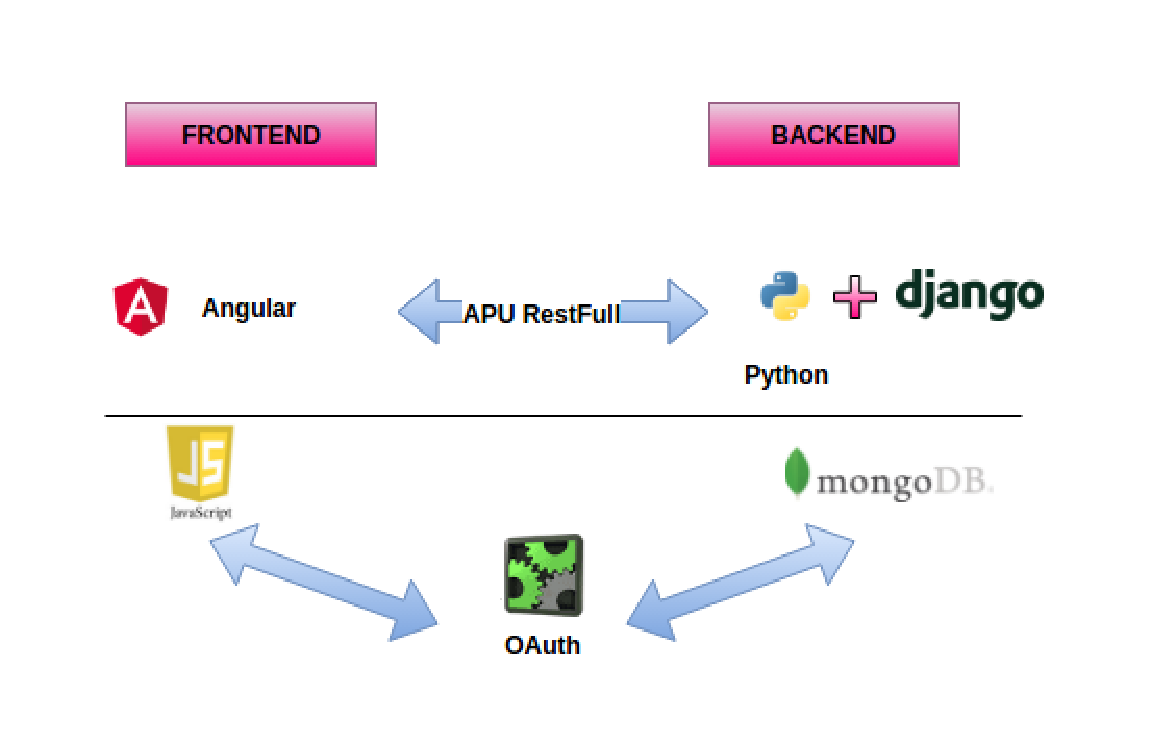
\includegraphics[scale=0.8]{resources/frontback.eps}

En el back encontramos la parte que no es visible en la aplicación, ahí de desarrolla la aplicación Python basada en Django. Django es un framework para el lenguaje Python que facilita el desarrollo de aplicaciones mediante diferentes componentes. Django pone énfasis en el re-uso, la conectividad y extensibilidad de componentes, el desarrollo rápido y el principio de no repetir código.  

Se necesita un almacenamiento en el cual tendremos la información referente a los usuarios que manejan la aplicación como los clientes y algunos datos de configuración. Dicho almacenamiento será NoSQL, de los diferentes tipos de base de datos que tenemos como NoSQL se va a utilizar mongodb. Mongodb es NoSQL y sus colecciones se basan en objetos JSON. Los datos que se utilizaran en la aplicación tienen un carácter sensible y están protegidos por la LOPD(Ley Orgánica de la protección de datos), por lo que se usará una codificación cifrada para prevenir ataques a dichos datos.

Respecto a la seguridad tenemos la parte de autenticación, la autenticación que se utilizará será OAuth. El protocolo OAuth nos permitirá conectarnos a la API de forma segura, se basa en un sistema simple para aplicaciones. Además este sistema protege la identidad del usuario y es utilizado en aplicaciones que usamos en nuestro día a día como Google, Facebook, Twitter, etc.

Conectando la parte de frontend y backend se tiene un API RestFull. API Rest es un medio unificado de intercambio de información, en nuestro caso se utilizada para hacer llamadas a la aplicación backend desde la parte de frontend.

El frontend, es parte visible al usuario en la que dispone de la una aplicación Javascript basada en Angular. AngularJS, es un framework de JavaScript de código abierto, mantenido por Google, que se utiliza para crear y mantener aplicaciones web de una sola página. Su objetivo es aumentar las aplicaciones basadas en navegador con capacidad de Modelo Vista Controlador (MVC), para hacer que el desarrollo y las pruebas sean más fáciles.

La aplicación tendrá acceso desde cualquier dispositivo en cualquier localización.Por otro lado presentará una experiencia de usuario que cumpla con la usabilidad y fácil interacción con el usuario de nuestra aplicación.

Englobando lo anterior recogemos que además se va a tratar de un sistema multiplataforma, que quiere decir que se podrá ejecutar en diferentes dispositivos(smartphone,desktop,tablet). Esta adaptación se realiza mediante páginas responsive, que adaptan la apariencia en función del dispositivo.

 






\section{Metodología y plan de trabajo}
Se muestra el siguiente diagrama de Gantt en el que se ven las fases que se van a seguir en el proyecto.Las tres fases correspondientes a aplicación web, API RestFull y aplicación backend. Además durante todo el trabajo se llevará a cabo una memoria explicativa.  

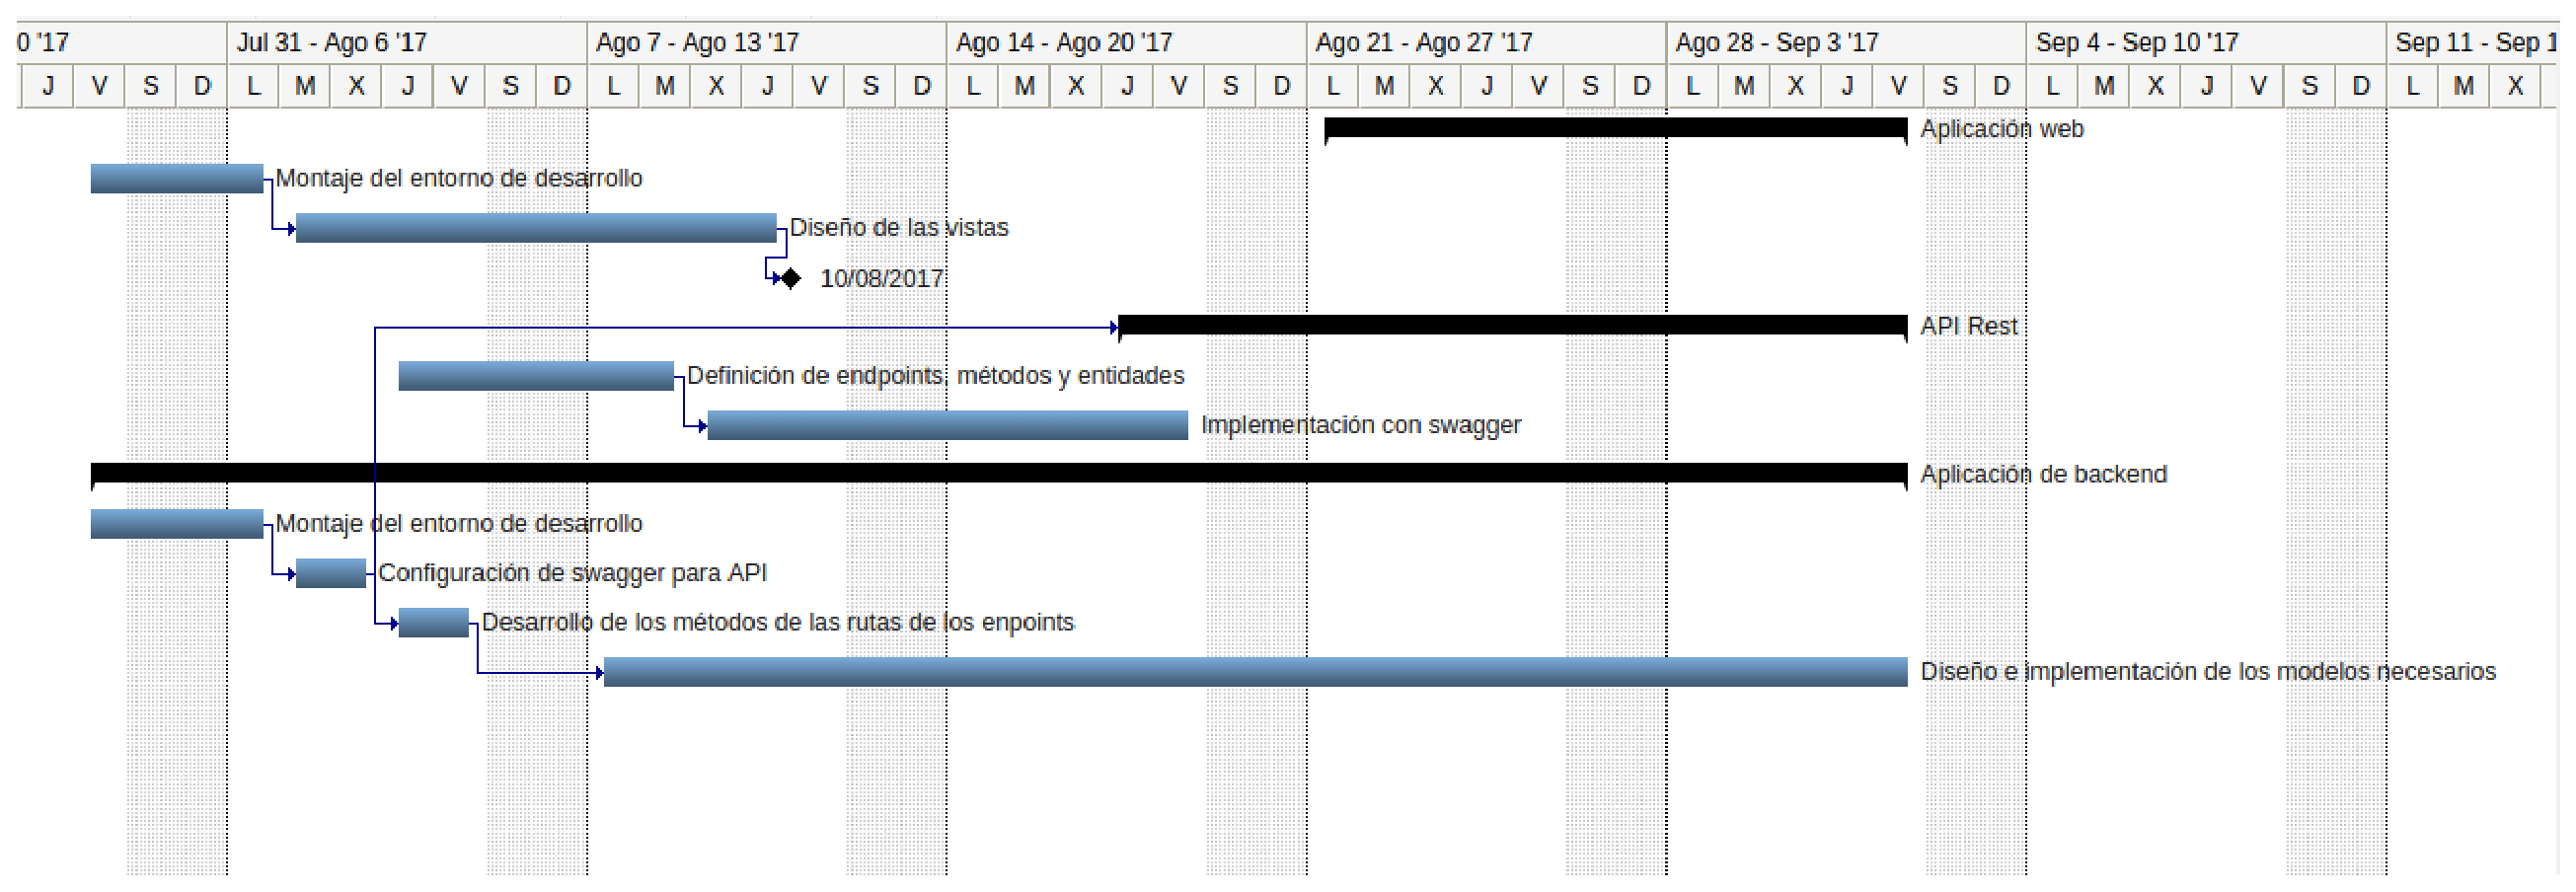
\includegraphics[scale=0.3]{resources/gantter.eps} 


\section{Medios}
Para el desarrollo del proyecto se va hacer uso de máquinas en Amazon, son máquinas virtuales en la nube.
El desarrollo del código se hará con el IDE PhpStorm y Pycharm. PhpStorm para el desarrollo de la parte de frontend que nos proporciona interfaz sencilla aunque no se programe en PHP. Por el otro lado PyCharm para el backend que se desarrollará en Python.

Todo el proyecto se encotrará en un repositorio GIT bajo control de versiones.

\section{Referencias}
\url{https://es.wikipedia.org/wiki/AngularJS}

\url{https://www.boe.es/buscar/act.php?id=BOE-A-2010-6737}

\url{https://es.wikipedia.org/wiki/Django_(framework)}





\nocite{*}
\bibliographystyle{plain}
\addcontentsline{toc}{section}{Referencias}


\end{document}
